\documentclass[a4paper]{article}
\usepackage{amsmath, mathtools, physics}
\usepackage{hyperref}
\usepackage{setspace}
\usepackage[margin=0.8in]{geometry}
\usepackage{xepersian}
\settextfont{B Zar}

\let\oldnorm\norm   % <-- Store original \norm as \oldnorm
\let\norm\undefined % <-- "Undefine" \norm
\DeclarePairedDelimiter\norm{\lVert}{\rVert}


\title{آموزش نصب جولیا }
\author{کارگاه جولیا انجمن عملی فیزیک شریف}
\date{اسفند ۱۴۰۰}

\begin{document}
	\maketitle
	\doublespacing
	در این نوشته قصد داریم به نصب جولیا و پکیچ های مورد نیاز در طول کارگاه بپردازیم.

	\section{نصب کامپایلر جولیا}
	 در قدم اول لازم است به سایت زیر مراجعه کنید:
	\begin{latin}
		\url{https://julialang.org/downloads} \\
	\end{latin}

	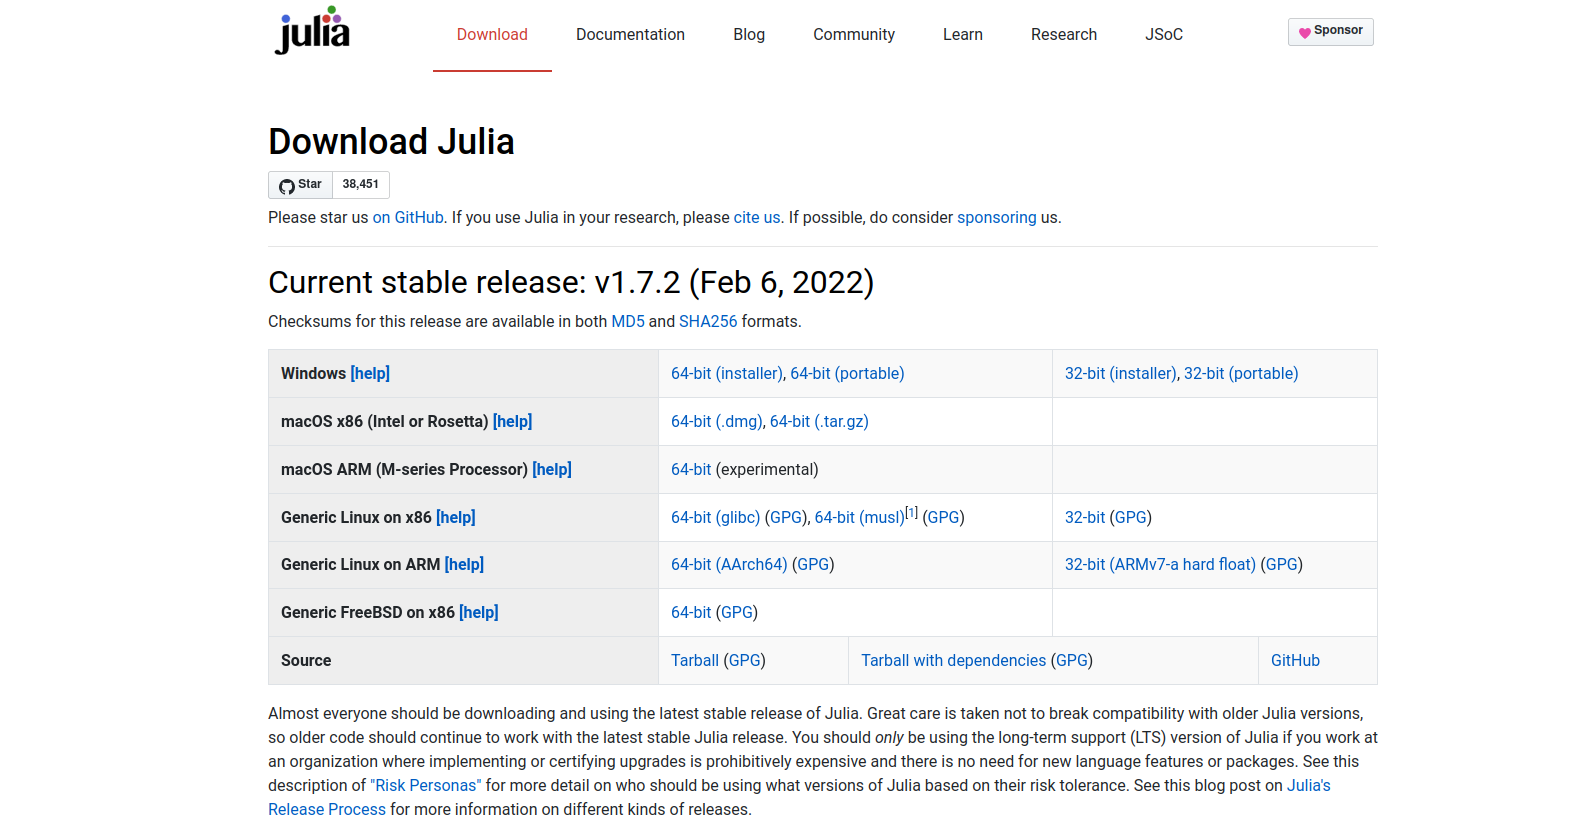
\includegraphics[width = \textwidth]{../img/img-1}

	در این بخش کافیست با انتخاب سیستم عامل خود و ۳۲ یا ۶۴ بیتی بودن آن، نسخه مناسب را بارگیری کنید.

	حال بعد از بارگیری فایل نصبی آن را اجرا کرده و فرایند نصب را طی کنید. توجه کنید که در زمانی که از شما درخواست شد، تیک گزینه \lr{Add Julia to PATH} فعال باشد.

	\begin{center}
		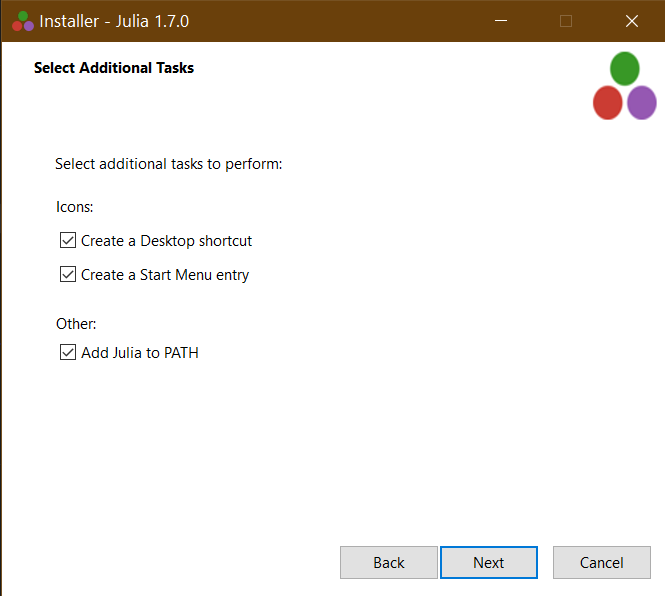
\includegraphics[height = \textheight/5]{../img/img-2} \\
	\end{center}
	 
	\textbf{نکته}: این گزینه برای کاربران ویندوز است. کاربران مک باید به کمک 
	\href{https://julialang.org/downloads/platform/#macos}{این لینک} به صورت دستی جولیا را به \lr{PATH} اضافه کنند. برای کاربران لینوکس نیز توصیه میشود که جولیا را از پکیج موجود در ریپازیتوری توزیع نصب کنند. \\

	با اتمام نصب، جولیا آماده راه اندازی است. کافیست محیط خط فرمان (\lr{CMD}) را راه اندازی کرده و در آنجا دستور \lr{julia} را اجرا کنید.

	نتیجه باید چیزی شبیه تصویر زیر باشد: \\\\

	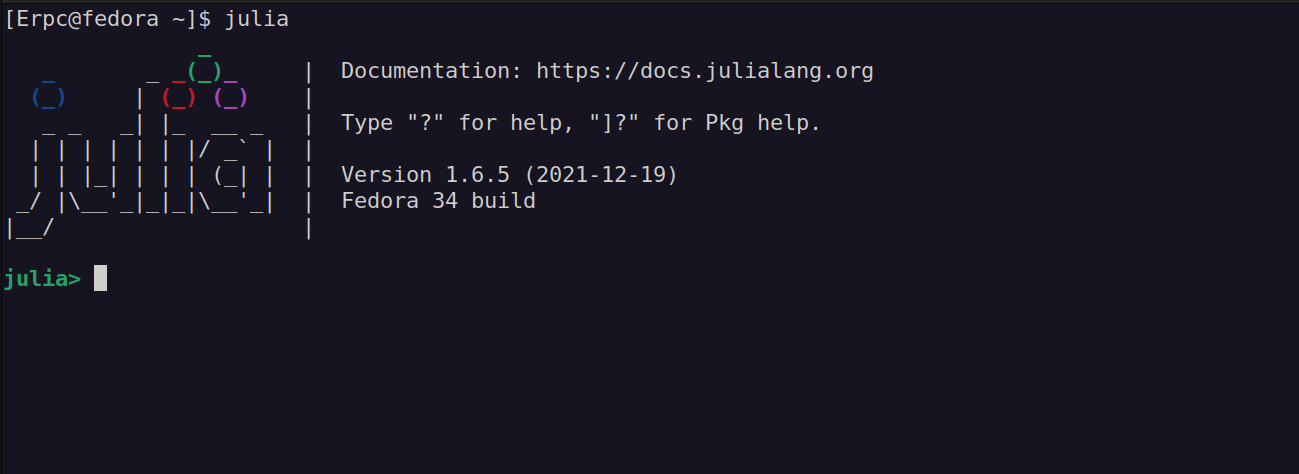
\includegraphics[width = \textwidth]{../img/img-3} \\

	 در این محیط میتوان دستورات مختلف جولیا را اجرا و امتحان کرد (برای مثال می‌توانید دستور \lr{pi} را اجرا کنید). 

	\section{نصب پکیج های مورد نیاز}
	نصب پکیج های جولیا توسط پکیج منیجر داخلی و در همین محیط انجام می‌شود. برای دسترسی به این پکیج منیجر کافیست کاراکتر براکت بسته " [ " را تایپ کنید. پس از این کار نشانک محیط به شکل زیر تغییر پیدا می‌کند: \\

	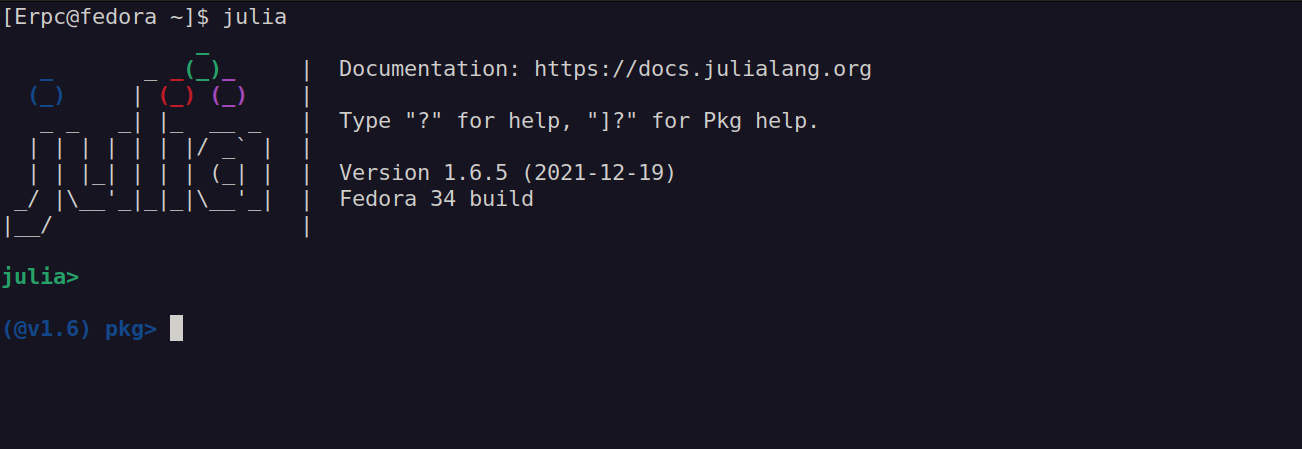
\includegraphics[width = \textwidth]{../img/img-4} \\

	.در محیط میتوان پکیج های مختلف جولیا را به کمک دستور \lr{add}  نصب کرد. برای مثال نصب پکیج \lr{LinearAlgebra} به صورت زیر است:\\

	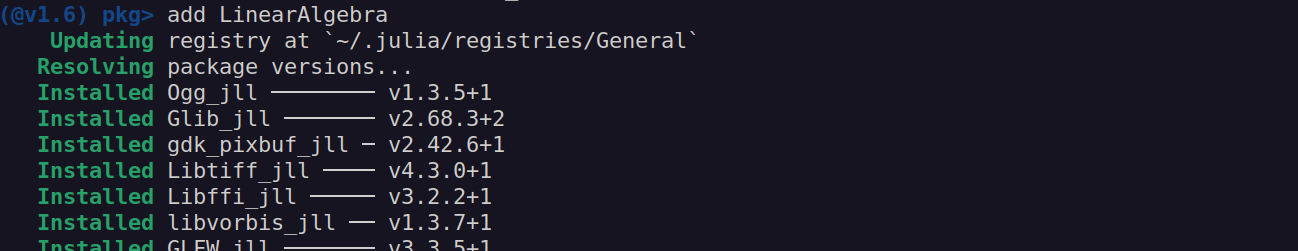
\includegraphics[width = \textwidth]{../img/img-5} \\

	با اتمام فرایند نصب، پکیج مورد نظر قابل استفاده در نرم افزار است.
	لیست پکیج های موردنیاز کارگاه در انتهای این فایل آورده شده.
\\
\textbf{نکته:} درصورتی که در فرایند نصب پکیجی با مشکل مواجه شدید، به کمک روشی که در ادامه آمده فایل های نصبی را پاکسازی کرده و مجددا تلاش به نصب پکیج کنید (استفاده از نرم افزار های رفع فیلتر نیز می‌تواند به حل بعضی از مشکلات نصب کمک کند).

	\subsection{استفاده دستور \lr{gc} برای پاکسازی پکیج های نصب نشده}

	در صورتی که در نصب پکیجی با مشکل مواجه باشید، استفاده از دستور \lr{gc} در محیط نصب پکیج می‌تواند مفید باشد:\\

	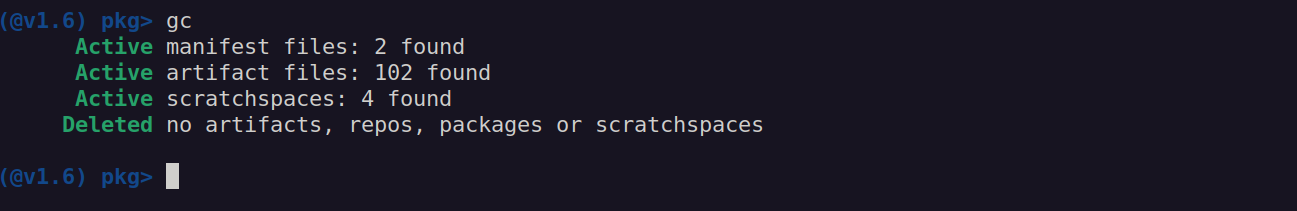
\includegraphics[width = \textwidth]{../img/img-6} \\

	با اجرای این دستور فایل های نصبی پکیج های ناموفق پاکسازی می‌شوند و میتوان به نصب مجدد آنها اقدام کرد.

	‌\section{ابزار های کمکی}

	 برای اجرای کد های جولیا کامپایلر این نرم‌افزار به تنهایی کافی است و می‌توانید با ایجاد فایلی با پسوند \lr{jl}
	 شروع به کد نویسی کتید. اما برای تجربه بهتر کدزنی استفاده از محیط های کدنویسی مانند \lr{VScode}
	 پیشنهاد می‌شود. در صورتی که از این محیط استفاده می‌کنید افزونه های \lr{Julia}
	 و \lr{Jupyter}
	 را نصب کنید و در صورتی که از محیط دیگری استفاده می‌کنید نیز نصب \lr{Jupyter} به تنهایی برای اجرای فایل های ارائه شده توسط کارگاه توصیه می‌شود. \\


	 در صورتی که در هر کدام از مراحل بالا به مشکلی برخوردید می‌توانید آن را در بخش کامنت پست کارگاه در کانال انجمن بیان کنید یا با مدرسین کارگاه از طریق ایمیل های زیر در ارتباط باشید. به امید دیدار دوباره در کارگاه :)
	\\ \\ ارمیا اعتمادی \quad \lr{epc1380@gmail.com}
	\\ یعقوب شاه‌ماری \quad \lr{shahmari.acer@gmail.com}
	\\ صالح شاملو \quad \lr{slhshamloo@gmail.com}
	  \\ \\
	لیست پکیج های مورد نیاز (موارد مهم بولد هستند): \\
	\lr{\textbf{Plots, LinearAlgebra, DiffrentialEquations.jl}, LaTeXStrings, Statistics, JLD, ProgressMeter} \\
	\lr{ProgressBars, StatsBase}
	\end{document}

